\documentclass{article} % For LaTeX2e
\usepackage[backend=bibtex, sorting=none]{biblatex}
\addbibresource{bibliography.bib}
\usepackage{nips15submit_e,times}
\usepackage{hyperref}
\usepackage{url}
\usepackage{amsmath}
\usepackage{tipa}
\usepackage{multicol}
\usepackage{multirow}
\usepackage{array}
\usepackage{graphicx}
\usepackage{bm}
\usepackage{mathtools,xparse}
\graphicspath{ {figures/} }
\newcolumntype{P}[1]{>{\centering\arraybackslash}p{#1}}
\usepackage[linesnumberedhidden,ruled,noend]{algorithm2e}
\usepackage{etoolbox}
\patchcmd{\abstract}{Abstract}{Project information}{}{}

\makeatletter
\def\BState{\State\hskip-\ALG@thistlm}
\makeatother
%\documentstyle[nips14submit_09,times,art10]{article} % For LaTeX 2.09

\title{COMPGI15: Information Retrieval and Data Mining Group Project - Report}

\author{
Sergiu Tripon\\
Department of Computer Science\\
University College London\\
Gower Street, London, WC1E\\
\texttt{sergiu.tripon.15@ucl.ac.uk}\\
\And
Santiago Gonzalez\\
Department of Computer Science\\
University College London\\
Gower Street, London, WC1E\\
\texttt{hernan.toral.15@ucl.ac.uk} \\
\And
Archie Norman \\
Department of Computer Science\\
University College London\\
Gower Street, London, WC1E\\
\texttt{archie.norman.15@ucl.ac.uk} \\
}

% The \author macro works with any number of authors. There are two commands
% used to separate the names and addresses of multiple authors: \And and \AND.
%
% Using \And between authors leaves it to \LaTeX{} to determine where to break
% the lines. Using \AND forces a linebreak at that point. So, if \LaTeX{}
% puts 3 of 4 authors names on the first line, and the last on the second
% line, try using \AND instead of \And before the third author name.

\newcommand{\fix}{\marginpar{FIX}}
\newcommand{\new}{\marginpar{NEW}}

\nipsfinalcopy % Uncomment for camera-ready version

\begin{document}

\maketitle

\section*{Project information}

The implementation code is available on GitHub at:

\url{https://github.com/santteegt/ucl-irdm-collaborative-filtering}

A manual is also available on GitHub at:

\url{https://github.com/santteegt/ucl-irdm-collaborative-filtering#user-content-collaborative-filtering-project-using-deep-learning}

\section{Introduction}

Nowadays, web enabled online services like e-stores and streaming platforms which offer an increasing amount of different products have been integrating Recommender Systems (RS) into their platforms aiming to make a more effective use of information. Recommender Systems play an important role by assisting customers to find products according to their taste over those platforms. Different approaches have been developed to provide accurate recommendations to users, however there has been a lack of data and research on the scope of music recommending systems.

Conventional methods use ratings given to items by users as the only source of recommendation. The prediction accuracy drops significantly when the ratings are very sparse. Moreover, they cannot be used for recommending new products which have yet to receive rating information from users. This is known as the "cold start" problem. Content information may be utilized, but loosely coupled methods process the auxiliary information once and then use it to provide features for the CF models (one-way interaction). Tightly coupled methods allow two-way interaction.

\section{Aim}

The aim of this group project is to develop and test a recommending system using two approaches: a pure probabilistic matrix factorization and a hierarchical Bayesian model using deep learning approach by employing the ratings (feedback) matrix and the related content information for learning stronger features. The recommender system will be evaluated in order to analyze how tightly coupled methods can automatically learn features from the auxiliary information and naturally balance the influence of the rating and the content information. The evaluation results of the implemented model will be compared with the baseline approach.

\section{Background \& Related work}

\subsection{Collaborative Topic Modeling for Recommending Scientific Articles}

Wang and Blei \cite{wang2011collaborative} developed an algorithm to recommend scientific articles to users of an online community. The algorithm combines the merits of traditional collaborative filtering and probabilistic topic modeling. It provides an interpretable latent structure for users and items, and can form recommendations about both existing and newly published articles, therefore tackling the cold start problem. The algorithm was evaluated against a large subset of data from CiteULike, a bibliography sharing service, which showed that the algorithm proposed provides a more effective recommender system than traditional collaborative filtering.

\subsection{A Hybrid GA-based Collaborative Filtering Model for Online Recommenders}

Ho et. al \cite{ho2007hybrid} created a Hybrid Genetic Algorithm-based Collborative Filtering MOdel applied on the MovieLens dataset. The model implements collaborative and content-based methods separately and then combines their predictions. It incorporates some content-based characteristics into a collaborative approach and some collaborative characteristics into a content-based approach. It also constructs a general unifying model that incorporates both content-based and collaborative characteristics. The model tackles the cold start problem occurring during the early period of usage, by adding an additional "preference" component which consists of features such as the user's preferred film type and language. This means that, during the early stage, the preference component will dominate the search function in the GA operation;

\subsection{Music recommendations using cover images}

A blog post by Eric Bernhardsson \cite{bernhardsson2014music} described an experiment which considered cover images as a means for music recommendations. The first attempt at recommendation involved resizing all image to 16x16, converting them to grayscale, subtracting the mean and normalizing by the variance, which resulted in fairly poor recommendations. A further attempt involved using pyleargist, a wrapper around a C library, which takes an image and outputs an image descriptor, which improved the recommendation results. According to Eric, the experiment's future work would involve learning a mapping from image space to collaborative filtering space and venturing into the realms of deep learning.

\subsection{Combining Spotify and Twitter Data for Generating a Recent and Public Dataset for Music Recommendation}

Pichl et al.'s research \cite{pichl2014combining} is based on the \#nowplaying dataset, the same dataset used in this project. Its aims were to implement and evaluate a pure collaborative filtering based recommender system. They found that for a high number of recommendations the recommender system was rather limited. During the evaluation phase, they discovered that further work was required. This included gathering of further context based information that is available such as time stamp or geolocation and implementing hybrid recommender system utilizing this additional context based information.

\subsection{Recommending music on Spotify with deep learning}

Sander Dieleman, a Spotify intern, wrote a blog post \cite{dieleman2014recommending} discussing his work on music recommendations using deep learning at Spotify. Dieleman's work focused on content-based music recommendation using convolutional neural networks. It involved training a model to predict the latent representations of songs that were obtained from a collaborative filtering model. This enabled the ability to predict the representation of a song in the collaborative filtering space, even if no usage data was available. If two songs are close together in this space, they are probably similar. If a song is close to a user, it is probably a good recommendation for that user, considering that they haven't listened to it yet. If predicting the position of a song in this space from audio is achieved, recommending the song to the right audience without having to rely on historical usage data can also be achieved.

\subsection{Collaborative Deep Learning for Recommender Systems}

Wang et al. \cite{wang2015collaborative} propose a a hierarchical Bayesian model called collaborative deep learning (CDL). CDL jointly performs deep representation learning for the content information and collaborative filtering for the ratings (feedback) matrix by using an stacked deep autoencoder model which is tightly coupled with a Collaborative Topic Model (CTR) in order to automatically learn features and balance them with the influence of ratings. Extensive experiments on three real-world datasets from different domains showed that CDL can significantly perform better than the state of the art.

\subsection{Types of Collaborative Filtering \cite{ho2007hybrid}}

\textbf{Content-based filtering}

As the name suggests, content-based filtering focuses on content. In a music-related context, a song will be recommended to a user if in the past the user has listened to another that shares the same genre as the song being recommended. Content-based filtering selects items based on the correlation between the content of the items and user preferences. For example, current search engines are based on automatic analysis of the content of documents and the content of user’s query. This type of filtering also bring disadvantages as the system can only recommend items scoring highly against the user profile. The user is restricted to see the items similar to those already rated and new items will never be recommended due to the working on an individual user.

\textbf{Item-based Collaborative Filtering}

Item-based Collaborative Filtering focuses on the similarity between the currently active user and other users. It aims to find new items the active user has never seen before but are predicted they would be interested in, based on other users' interest in the items. For example, users A, B and C all like Item 1. Two of the users, A and B also like Item 3. Item 3 would then be recommended to user C based on user A and B's interest in the item. The similarity can either be measured by the same item which is known as item-based CF or by the same type of user, which is known as user-based CF. This method is quite common for current recommendation systems, which have been wildly used by MovieLens and Yahoo. Item-based techniques first analyze a user-item matrix to identify relationships between different items, and then use these relationships to indirectly compute recommendations for users.

\textbf{User-based Collaborative Filtering}

User-based Collaborative Filtering is similar to item-based CF with the difference being that it looks at similarities between users rather than items. For example, User A likes Item 1, 2 and 4. User B likes Item 1 and 2. Items 1 and 2 are common between User A and B. Therefore, Item 4 will be recommended to User B as User A and B are deemed as like-minded users.

\section{Data}

For this project, we use as main data sources the \#nowplaying dataset \cite{zangerle2014nowplaying} and the public MusicBrainz\footnote{\url{https://musicbrainz.org/}} music encyclopedia for music metadata. The former is a social media-based dataset which combines Twitter and Spotify data in order to create a relationship indicating music listening behaviour of Twitter users. The authors attempted to find a match between the user's Twitter and Spotify user names. If the user names were identical, a match was found and that user's data was kept in the dataset. In the situation where a match was not found, the data was discarded in order to preserve data quality and accuracy. The dataset also provides Artist and Track IDs for the MusicBrainz database. Using these identifiers provided, we are able to extract further artist and track-related features which boosts recommendation accuracy.

\subsection{Dataset analysis}

Table \ref{table:1} presents number of tweets, users, tracks and artists in the \#nowplaying dataset dump downloaded on 06/04/2016.

\begin{table}[!htbp]
\caption{Number of tweets, users, tracks and artists in the dataset as of 06/04/2016.}
\label{table:1}
\begin{center}
\begin{tabular}{l l l l}
\multicolumn{1}{c}{\bf Tweets} & \multicolumn{1}{c}{\bf Users} & \multicolumn{1}{c}{\bf Artists} & \multicolumn{1}{c}{\bf Tracks}
\\ \hline \\
88,745,248 & 5,497,005 & 151,440 & 772,485\\
\end{tabular}
\end{center}
\end{table}

Table \ref{table:2} showcases the top 5 most popular sources used by the users in the \#nowplaying dataset as of 06/04/2016.

\begin{table}[ht]
\caption{Top 5 most popular sources as of 06/04/2016.}
\label{table:2}
\begin{center}
\begin{tabular}{l l l l}
\multicolumn{1}{c}{\bf Source} & \multicolumn{1}{c}{\bf Times used}
\\ \hline \\
Securenet Systems Radio Playlist Update & 13,326,642\\
Spotify                                 & 7,132,339\\
Web                                     & 4,139,372\\
SAM Broadcaster Song Info               & 3,439,207\\
BigUrl                                  & 3,170,726\\
%Twitter for iPhone                      & 3,080,571\\
%Twitter for Android                     & 2,348,784\\
%Share.Radionomy.com                     & 2,342,915\\
%iOS                                     & 2,257,604\\
%Wavepanel                               & 1,809,559\\
\end{tabular}
\end{center}
\end{table}

Table \ref{table:3} presents the top 5 most popular tracks listened to by the users in the \#nowplaying dataset as of 06/04/2016.

\begin{table}[!htbp]
\caption{Top 5 most popular tracks as of 06/04/2016.}
\label{table:3}
\begin{center}
\begin{tabular}{l l l l}
\multicolumn{1}{c}{\bf Artist} & \multicolumn{1}{c}{\bf Track} & \multicolumn{1}{c}{\bf Times played}
\\ \hline \\
ON              & Generations                & 934,021\\
NP              & B4                         & 597,004\\
Rihanna         & Should I?                  & 331,434\\
Coldplay        & Swallowed in the Sea       & 327,967\\
Taylor Swift    & Crazier                    & 264,918\\
%Katy Perry      & ET                         & 257,538\\
%Bruno Mars      & Talking to the Moon        & 251,635\\
%Michael Jackson & Can't Let Her Get Away      & 251,444\\
%One Direction   & Total Eclipse of the Heart & 249,959\\
%U2              & Salome                     & 245,442\\
\end{tabular}
\end{center}
\end{table}

\subsection{Sample Extraction}

During the data analysis phase of the project, we discovered that the data was too large for the computational power we had available. This lead to the decision of extracting a sample from the data set. For this, we used the following workflow for extracting a sample data set for training/validating our models:

\begin{enumerate}
    \item Aggregate the data and calculate each users tweet count (No. of songs published)
    \item Filter users with 3 or more tweets
    \item Extract a sample of 100.000 records using reservoir sampling
    \item Calculate basic statistics such as number of users and tracks, and mean and standard deviation of the number of publications (items) per user.
\end{enumerate}

Table \ref{table:4} presents stats of the extracted sample such as number of users and tracks, mean and standard deviation. Further explanation regarding to the sampling method used for this task is exposed in the following section.

\begin{table}[!htbp]
\caption{Stats of the extracted sample data set.}
\label{table:4}
\begin{center}
\begin{tabular}{c c c c}
\multicolumn{1}{c}{\bf Users} & \multicolumn{1}{c}{\bf Tracks} & \multicolumn{1}{c}{\bf Mean} & \multicolumn{1}{c}{\bf Std. Deviation}
\\ \hline \\
35,122 & 49,679 & 2.8 & 16.1\\
\end{tabular}
\end{center}
\end{table}

\subsection{Reservoir Sampling}

Reservoir Sampling \cite{reservoirsampling} is a collection of randomized algorithms used to choose a random sample of \textit{k} items from a list S containing \textit{n} items, in the context where \textit{n} is a very large or unknown number. Typically, \textit{n} is large enough for it to not fit into main memory. The pseudo-code for Reservoir Sampling:

\begin{itemize}
    \item Keep the first item in memory.
    \item When the \textit{i}-th item arrives (for \textit{i} \textgreater 1):
    \item with probability $ 1 / i $, keep the new item instead of the current item;
    \item with probability $ 1-1 / i $, keep the current item and discard the new item.
\end{itemize}

So:

\begin{itemize}
    \item when there is only one item, it is kept with probability 1;
    \item when there are 2 items, each of them is kept with probability $ 1/2 $;
    \item when there are 3 items, the third item is kept with probability $ 1/3 $, and each of the previous 2 items is also kept with probability $ (1/2)(1-1/3) = (1/2)(2/3) = 1/3 $;
    \item by induction, it is easy to prove that when there are \textit{n} items, each item is kept with probability $ 1/n $.
\end{itemize}

Figure \ref{fig:samplingP} shows the transformation schema used in Pentaho to getting a sample from the now playing data set that has users with 3+ published items.

\begin{figure}[ht]
\centering
\fbox{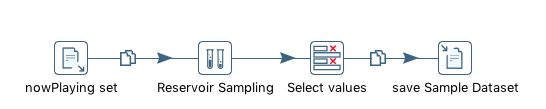
\includegraphics[scale=0.6]{figures/sampling}}
\caption{Reservoir Sampling in Pentaho: Data Integration Platform.}
\label{fig:samplingP}
\end{figure}

\subsection{Data Integration for content extraction}

In order to integrate the nowplaying sample set with the content information of each track from MusicBrainz, another transformation was built in Pentaho to obtain the list of user-tracks ids. Figure \ref{fig:forRatrings} outlines the flow diagram of the transformation, where only the track-based output was used in our project as it can be also used to obtained the artist content information. The obtained output file was used to obtain the content information from the MusicBrainz Postgres Database, as well as the required files to generate the rating matrix for the CTR matrix factorization model. The generated files can be found under the \textit{data} folder in project repository.

\begin{figure}[ht]
\centering
\fbox{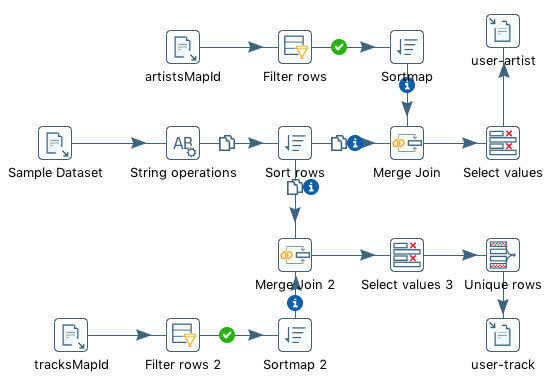
\includegraphics[scale=0.6]{figures/forRatings}}
\caption{Mapping of nowPlaying/MusicBrainz Ids for content extraction and rating matrix construction}
\label{fig:forRatrings}
\end{figure}

\subsection{Ratings Matrix generation}

A ratings matrix was generated, consisting of the entire collection of items in the sample data set to give a J by S matrix X. We generated a binary matrix whereby if the user has listened to a track we assign a value of 1, while if they haven't listened to the track, we assign 0. Two files were generated, output\_by tracks and output\_by\_user. Each file aggregates each item and associates the user\_id or track\_id in the corresponding row. Tables \ref{table:5} and \ref{table:6} present an example of the format of each file generated.

\begin{table}[!htbp]
\caption{Aggregated tracks played per user.}
\label{table:5}
\begin{center}
\begin{tabular}{c c c c}
\textbf{user\_id} & \textbf{count} & \textbf{track\_id} & \textbf{track\_id}\\
693afc22f9b838a38... & 2 & 013d1e71\-f6a4\-3adc... & dcca7fcb\-aa17\-36d5...\\
ba6b4825ca63356b0... & 2 & 006cddf7\-52f3\-3eb8... & 001c124e\-c675\-3b0c...\\
\end{tabular}
\end{center}
\end{table}

\begin{table}[!htbp]
\caption{Aggregated users played per track.}
\label{table:6}
\begin{center}
\begin{tabular}{c c c c}
\textbf{track\_id} & \textbf{count} & \textbf{user\_id} & \textbf{user\_id}\\
114fd187\-dfed\-3fcd... & 2 &  662ed5aa9df25a7b43... &  663jd5aa9df25a3b...\\
063ed02c\-53d8\-3fd2... & 2 &  aae7d3b35d7fca7be0... &  762ed56aa9d65a7b...\\
\end{tabular}
\end{center}
\end{table}

\section{Technological Stack}

\subsection{Google: TensorFlow\texttrademark}

"TensorFlow\texttrademark is an open source software library for numerical computation using data flow graphs. Nodes in the graph represent mathematical operations, while the graph edges represent the multidimensional data arrays (tensors) communicated between them. The flexible architecture allows you to deploy computation to one or more CPUs or GPUs in a desktop, server, or mobile device with a single API." \cite{tensorflow}

\subsection{Dato: GraphLab Create}

"GraphLab Create is an extensible machine learning framework that enables developers and data scientists to easily build and deploy intelligent applications and services at scale. It includes distributed data structures and rich libraries for data transformation and manipulation, scalable task-oriented machine learning toolkits for creating, evaluating, and improving machine learning models, data and model visualization for all aspects of development, and a client to define and deploy both distributed batch jobs to Dato Distributed™ as well as real-time machine learning services to Dato Predictive Services™. It is designed for end-to-end developer productivity, scale, and the variety and complexity of real-world data." \cite{graphlabcreate}

\subsection{Pentaho: Data Integration}

"Pentaho Data Integration prepares and blends data to create a complete picture of your business that drives actionable insights. The platform delivers accurate, analytics-ready data to end users from any source. With visual tools to eliminate coding and complexity, Pentaho puts big data and all data sources at the fingertips of business and IT users." \cite{pentahodataintegration}

\section{Methodology}

\subsection{Item Similarity Model}

The item similarity model calculates the similarity between items using the historical data representing the interaction between the users and the tracks. Based on the similarity between track \textit{a} and \textit{b}, it recommends a track \textit{c} for user \textit{u} using a weighted average of the user's previous interactions.

Because the \#nowplaying dataset does not consist of rating information, the item similarity model uses Jaccard similarity to calculate the similarity between two tracks, which is an ideal choice when the information available only indicates whether the user listened to a song or not and not the rating a user awarded a song.

Jaccard similarity can be used to measure the similarity between two sets of tracks. In this model, calculating the Jaccard similarity between two tracks is achieved as follows:

\begin{equation}
    JS(a,b) = \frac{|U_a \cap U_b|}{|U_a \cup U_b|}
\end{equation}

where \textit{U\textsubscript{i}} is the set of users who listened to track \textit{i}.

\subsection{Popularity-based Recommender Model}

The Popularity-based Recommender Model determines a track's overall popularity and ranks the track based on it. The a track is recommended to a user, the track is scored based on the number of times it appears in the dataset. In this model, the track scores are identical for all users, which means the Popularity Recommender Model does not provide tailored recommendations. However, it can be used as a model for new users in an attempt to tackle the "cold start" problem.

\subsection{Factorization Recommender for Ranking Model}

The Factorization Recommender for Ranking model aims to learn latent factors for each user and track and uses the factors to rank recommendations in terms of the likelihood of observing (user, track) interactions.

\subsection{Collaborative Deep Learning (CDL) Model}

The Collaborative Deep Learning model is a novel tightly coupled method for Recommending Systems based on the Stacked Denoising Auto-Encoder (SDAE) deep learning model. Its basic version uses a bag-of-words representation for content features, where the CDL can simultaneously extract an effective deep feature representation from content and capture the similarity and relationship between items and users. Additionally, the deep autoencoder can be easily extended to incorporate other auxiliary information to further boost the performance.

Figure \ref{fig:cdlworkflow} describes each section of the proposed model. Our implementation is based on the Matlab code created by Wang et. al. \cite{wang2015collaborative} and the deep autoencoder implementation in Tensorflow presented by Green \cite{christofergreen2016}. First, an unsupervised pre-training is performed one layer at a time by minimizing the (cross-entrophy) error in reconstructing the input. Then, the middle layer $X_{L/2}$ serves as a bridge between the ratings and content information, being the key that enables CDL to simultaneously learn an effective feature representation and capture the similarity items. Finally, once all layers are pre-trained, the network goes through a second stage of training or supervised-fine-tuning, where the prediction error is to be minimized. 

\begin{figure}[!htbp]
\begin{center}
\fbox{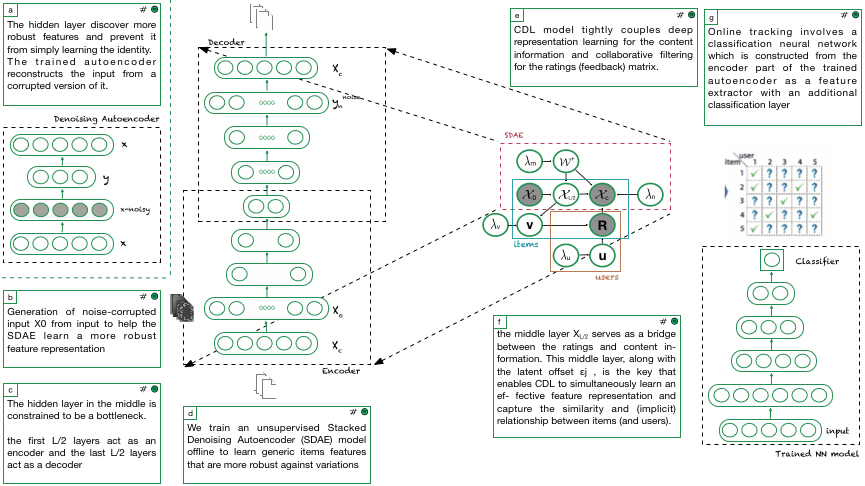
\includegraphics[width=13.7cm]{figures/cdl}}
\end{center}
\caption{Collaborative Deep Learning Model workflow.}
\label{fig:cdlworkflow}
\end{figure}

\section{Evaluation}

For evaluating our baseline recommender systems, we select 3/4 of the extracted sample data and set it as the training set while the remaining data is set as the test set. We use recall as the performance measure as the rating information is in the form of implicit feedback. Figure  \ref{fig:recalleval} presents the evaluation of recall over the top K items with K=10, and where results are averaged over all users. The rank factorization model is considered the most stable and better model as the recall increases with the number of top recommendations needed. Althought the popularity model performs better for K\textgreater6 but lower it is unstable for lower values of K as the recall value fluctuates. Additionally, the mean average precision was also evaluated for each model. Figure \ref{fig:mapeval} outlines once again the the factorization model is more stable with increasing K.

\begin{figure}[!hbtp]
\begin{center}
\fbox{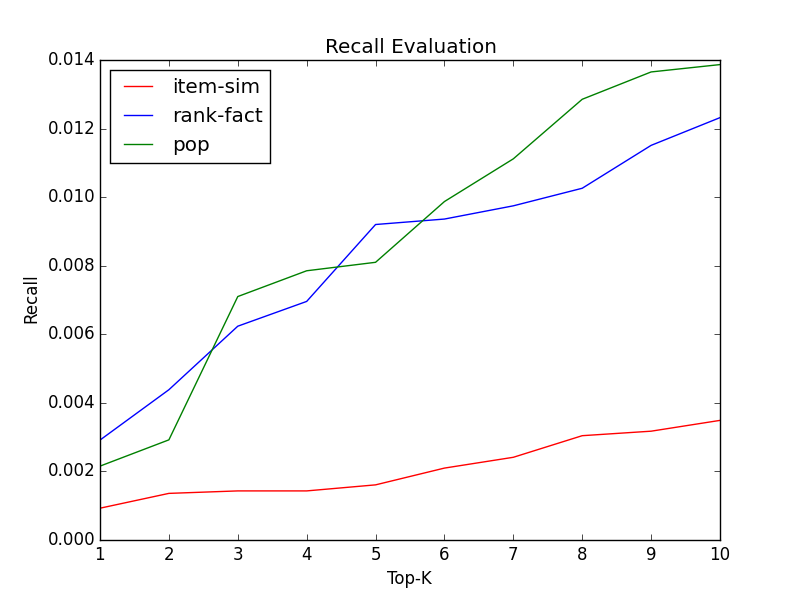
\includegraphics[width=13.1cm]{figures/recall}}
\end{center}
\caption{Recall Evaluation over Top-K items.}
\label{fig:recalleval}
\end{figure}

\begin{figure}[!htbp]
\begin{center}
\fbox{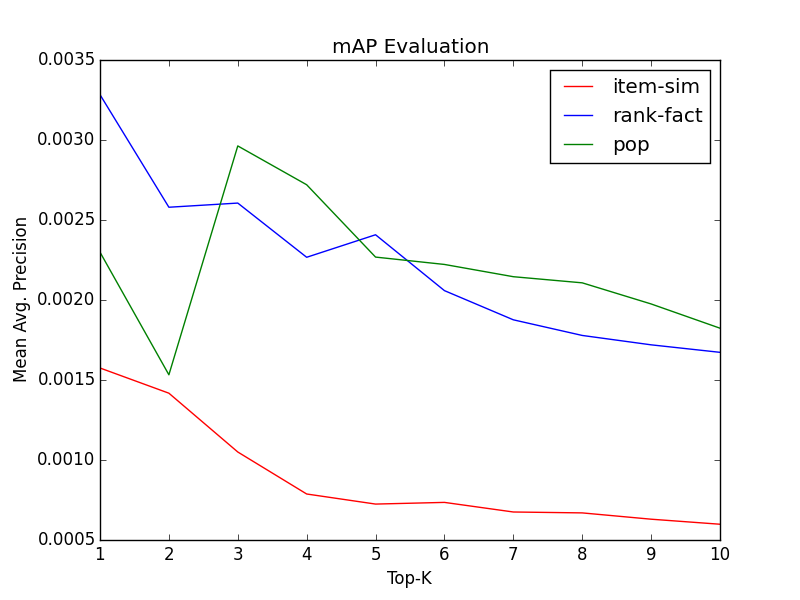
\includegraphics[width=13.1cm]{figures/map}}
\end{center}
\caption{Mean Average Precision Evaluation over Top-K items.}
\label{fig:mapeval}
\end{figure}

\section{Results}

\subsection{Item Similarity Model}

When run, the Item Similarity Model recommends 10 tracks for each user. Additionally, using the model, similar tracks can also be retrieved. Table \ref{table:7} presents an example of 5 track recommendations generated by the Item Similarity Model, with Rock being a predominant genre. Table \ref{table:8} presents an example of 5 similar tracks generated by the Item Similarity Model, indicating poor similarity accuracy.

\begin{table}[!htbp]
\caption{Example of 5 track recommendations generated by the Item Similarity Model.}
\label{table:7}
\begin{center}
\begin{tabular}{l l l}
\multicolumn{1}{c}{\bf Artist} & \multicolumn{1}{c}{\bf Track} & \multicolumn{1}{c}{\bf Genre}
\\ \hline \\
James Morrison & You Make It Real     & Pop Rock\\
Prefab Sprout & King of Rock and Roll & Pop, Rock, Sophisti-Pop\\
Curtis Stigers & I Wonder Why         & Jazz, Soft Rock\\
Westlife & You Raise Me Up            & Pop\\
Toto & I'll Be Over You               & Soft Rock\\
\end{tabular}
\end{center}
\end{table}

\begin{table}[ht]
\caption{Example of 5 similar tracks generated by the Item Similarity Model.}
\label{table:8}
\begin{center}
\begin{tabular}{p{2cm} p{4.6cm} p{2cm} p{2.5cm}}
\multicolumn{1}{c}{\bf Track} & \multicolumn{1}{c}{\bf Similar Track} & \multicolumn{1}{c}{\bf Track Genre} & \multicolumn{1}{c}{\bf Similar Track Genre}
\\ \hline \\
Iris by Iris & Rockstar by Nickelback & Hard Rock & Southern Rock\\
Iris by Iris & Antenna by Fuse ODG & Hard Rock & Afrobeats, Dance\\
Iris by Iris & All I Wanna Do by Sheryl Crow & Hard Rock & Pop\\
Iris by Iris & Vertigo by Vertigo & Hard Rock & Alternative rock\\
Iris by Iris & Boomerang by Boomerang & Hard Rock & Electronic, Latin, Funk/Soul, Pop\\
\end{tabular}
\end{center}
\end{table}

\subsection{Popularity-based Recommender Model}

When run, the Popularity-based Recommender Model recommends 10 tracks for each user. Additionally, using the model, similar tracks can also be retrieved. Table \ref{table:9} presents an example of 5 track recommendations generated by the Popularity-based Recommender Model, with Electronic being a predominant genre. Table \ref{table:10} presents an example of 5 similar tracks generated by the Popularity-based Recommender Model, indicating significantly poor similarity accuracy.

\begin{table}[!htbp]
\caption{Example of 5 track recommendations generated by the Popularity-based Recommender Model.}
\label{table:9}
\begin{center}
\begin{tabular}{l l l}
\multicolumn{1}{c}{\bf Artist} & \multicolumn{1}{c}{\bf Track} & \multicolumn{1}{c}{\bf Genre}
\\ \hline \\
ON              & I               & Electronic, Rock\\
NP              & I               & Electronic\\
A               & A               & Alternative Rock\\
Ne              & Yo              & Electronic\\
Various Artists & Various Artists & N/A\\
\end{tabular}
\end{center}
\end{table}

\begin{table}[!htbp]
\caption{Example of 5 similar tracks generated by the Popularity-based Recommender Model.}
\label{table:10}
\begin{center}
\begin{tabular}{p{2.8cm} p{4cm} p{1.5cm} p{3cm}}
\multicolumn{1}{c}{\bf Track} & \multicolumn{1}{c}{\bf Similar Track} & \multicolumn{1}{c}{\bf Track Genre} & \multicolumn{1}{c}{\bf Similar Track Genre}
\\ \hline \\
2 Times by Ann Lee & Io non sono qui by Ushas & Eurodance & Hard Rock\\
2 Times by Ann Lee & Cinta Jangan Kau Pergi by Sheila Majid & Eurodance & Jazz, Funk/Soul, Pop\\
2 Times by Ann Lee & Seal Your Fate by Obituary & Eurodance & Rock\\
2 Times by Ann Lee & No Man Is an Island by Tenth Avenue North & Eurodance & Rock, Pop\\
2 Times by Ann Lee & My Life by Richie Spice & Eurodance & Reggae\\
\end{tabular}
\end{center}
\end{table}

\subsection{Factorization Recommender for Ranking Model}

When run, the Factorization Recommender for Ranking Model recommends 10 tracks for each user. Additionally, using the model, similar tracks can also be retrieved. Table \ref{table:11} presents an example of 5 track recommendations generated by the Factorization Recommender for Ranking Model, with Rock being somehow a predominant genre. Table \ref{table:12} presents an example of 5 similar tracks generated by the Factorization Recommender for Ranking Model, indicating poor similarity accuracy.

\begin{table}[!htbp]
\caption{Example of 5 track recommendations generated by the Factorization Recommender for Ranking Model.}
\label{table:11}
\begin{center}
\begin{tabular}{l l l}
\multicolumn{1}{c}{\bf Artist} & \multicolumn{1}{c}{\bf Track} & \multicolumn{1}{c}{\bf Genre}
\\ \hline \\
A            & A                 & Alternative Rock\\
Ne           & Yo                & Electronic\\
Ed Sheeran   & She               & Folk\\
Black Cherry & Acid Black Cherry & Rock\\
Ten Sharp    & Stay              & Pop Rock, Prog Rock\\
\end{tabular}
\end{center}
\end{table}

\begin{table}[!htbp]
\caption{Example of 5 similar tracks generated by the Factorization Recommender for Ranking Model.}
\label{table:12}
\begin{center}
\begin{tabular}{p{2.2cm} p{3.6cm} p{3.2cm} p{3.3cm}}
\multicolumn{1}{c}{\bf Track} & \multicolumn{1}{c}{\bf Similar Track} & \multicolumn{1}{c}{\bf Track Genre} & \multicolumn{1}{c}{\bf Similar Track Genre}
\\ \hline \\

Just Say Yes by Snow Patrol & It's Raining Men by The Weather Girls & Synthpop, Electronica & Hi-NRG, Post-disco\\
Just Say Yes by Snow Patrol & Catfish Blues by Robert Petway & Synthpop, Electronica & Blues\\
Just Say Yes by Snow Patrol & Amor Depredador by The Mills & Synthpop, Electronica & Latin Rock, Alternative rock\\
Just Say Yes by Snow Patrol & Damn It Feels Good to Be a Gangsta by Geto Boys & Synthpop, Electronica & Gangsta Rap, Southern Hip Hop, Horrorcore\\
Just Say Yes by Snow Patrol & Walking On The Sun by Smash Mouth & Synthpop, Electronica & Ska Pop, Psychedelic Rock\\

\end{tabular}
\end{center}
\end{table}

\subsection{Collaborative Deep Learning (CDL) Model}

Because of the limited time period we had available to finish this assignment, we were not able to finish the integration of the deep autoencoder implementation with the rating matrix factorization (the latter is an implementation of Wang et. al.\cite{wang2015collaborative}). However, in our GitHub repository, we include the developed code using TensorFlow in the \textit{cdl} folder, where we set up a Stacked Denoising Autoencoder configured with 2 hidden layers of 200 and 50 neurons, a dropout module to learn stronger features, and a Gradient Descent optimizer, even though a Momentum optimizer would be a better algorithm (easy to use in TensorFlow) that can be used to alleviate the local optimum problem.

\section{Future Work}

As CDL is actually a more general framework which can also admit other deep learning models, a further investigation could be done on integrating the current solution with existing models such as Boltzmann machines, Recurrent Neural Networks, and Convolutional Neural Networks. Additionally, refining the feature representation by adding audio signals from track previews to boost the prediction accuracy, as applied by Spotify \cite{van2013deep} is another potential future focus.

\clearpage
\printbibliography
\end{document}